\documentclass[12pt]{article}
\usepackage[utf8]{inputenc}
\usepackage[greek,english]{babel}
\usepackage{alphabeta}
\usepackage{fancyhdr}
\usepackage{listings}
\usepackage{mathtools}
\usepackage{xcolor}
\usepackage{float}
\usepackage{siunitx}
\usepackage[margin=0.5in]{geometry}
\usepackage[backend=bibtex]{biblatex}

\title{Εργαστήριο Μικροηλεκτρονικής -- Εργασία 3}
\author{Χρήστος Μαργιώλης -- 19390133}
\date{Μάιος 2022}

\begin{document}

\begin{titlepage}
        \maketitle
        \begin{figure}[t!]
        \begin{center}
        
\includegraphics[scale=0.3]{./res/uniwalogo.png} \\
        \Large
        \textbf{Πανεπιστήμιο Δυτικής Αττικής} \\
        \large
        Τμήμα Μηχανικών Πληροφορικής και Ηλεκτρονικών Υπολογιστών
        \end{center}
        \end{figure}
\end{titlepage}

\renewcommand{\contentsname}{Περιεχόμενα}
\tableofcontents
\pagebreak

\section{Θεωρητικό μέρος}

Η εργαστηριακή άσκηση αυτή έχει ως θέμα τον αναλογικό αθροιστή. Το κύκλωμα και
η συμπεριφορά του είναι παρόμοια με αυτή του αναστρέφοντα ενισχυτή, απλώς με
περισσότερα σήματα εισόδου. Ο αθροιστής χρησιμοποιείται κυρίως σε κυκλώματα
μετατροπής ψηφιακού σήματος σε αναλογικό (digital to analog converter). Η
είσοδος και η έξοδος έχουν πάντα $\pi$ ($\SI{180}{\degree}$) διαφορά φάσης.

Ζητούμενο της εργαστηριακής άσκησης είναι να υλοποιήσουμε έναν 4bit μετατροπέα
BCD σε αναλογικό.

\section{Υλοποίηση της εργασίας}

Για την υλοποίηση της εργασίας χρησιμοποιήθηκαν τα παρακάτω εργαλεία:
\begin{itemize}
	\item Tina-TI για την συνδεσμολογία και τις μετρήσεις του κυκλώματος.
	\item Tinkercad για την υλοποίηση του κυκλώματος σε breadboard.
	\item \LaTeX για την συγγραφή της εργασίας.
\end{itemize}

\section{Συνδεσμολόγηση κυκλώματος}

\begin{itemize}
	\item Συνδεσμολογήστε το παρακάτω κύκλωμα με $V_1 = \SI{15}{\volt}$,
		$V_2 = \SI{-15}{\volt}$.
\end{itemize}

Παρατηρούμε ότι το κύκλωμα είναι ένας αθροιστής (αριστερό μέρος) και ένας
αναστρέφων ενισχυτής (δεξί μέρος).

\begin{figure}[H]
	\centering
	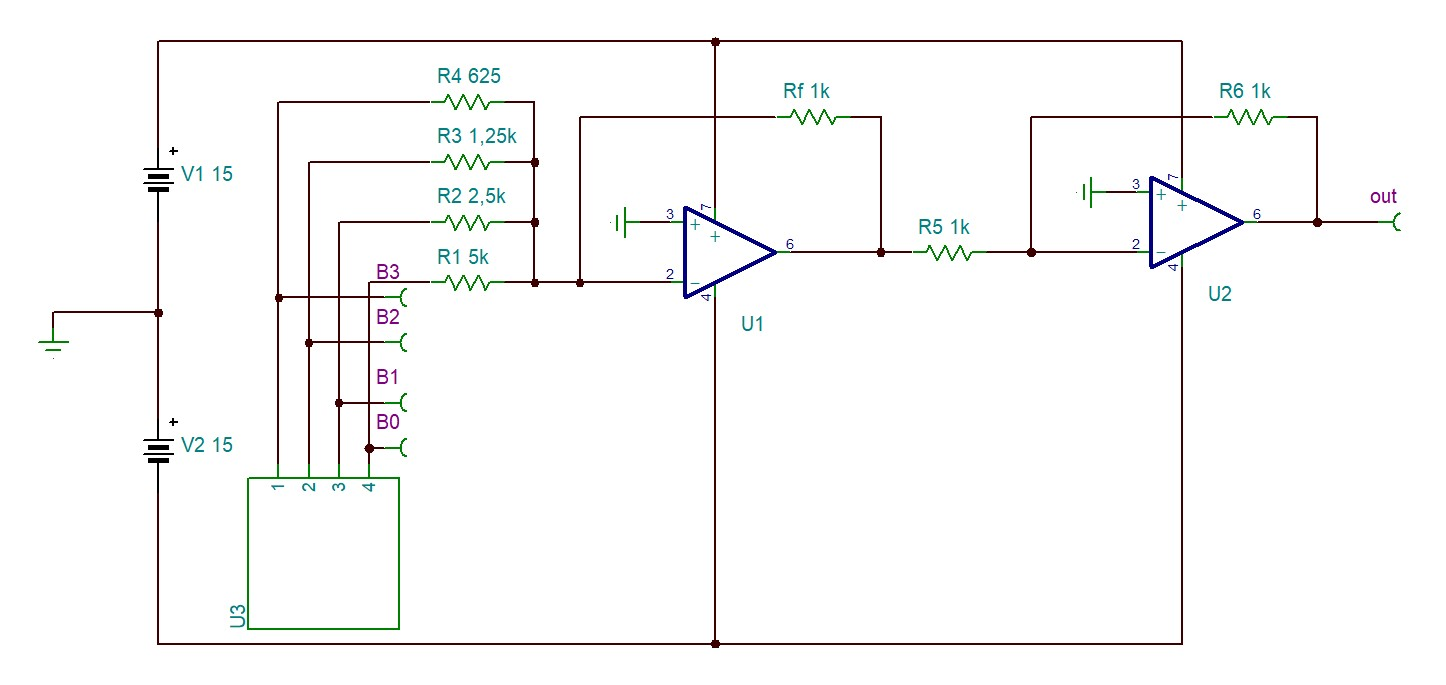
\includegraphics[width=\linewidth]{./res/schem_theor.jpg}
	\caption{4bit μετατροπέας BCD σε αναλογικό με θεωρητικές αντιστάσεις}
\end{figure}

\section{Εφαρμογή σήματος}

\begin{itemize}
	\item Εφαρμόστε το κατάλληλο ψηφιακό σήμα στις εισόδους του κυκλώματος
		σύμφωνα με το BCD.
	\begin{itemize}
	\item Υπολογίστε τις αντιστάσεις που απαιτούνται θεωρητικά για την
		λειτουργία του κυκλώματος.
	\item Επιλέξτε από τον πίνακα «τυπικές τιμές αντιστάσεων» τις
		αντιστάσεις που προσεγγίζουν τις θεωρητικές.
	\item Συμπληρώστε τον πίνακα εξόδου.
	\item Αναπαραστήστε σε γράφημο την έξοδο του κυκλώματος ως προς την
		είσοδο.
	\end{itemize}
\end{itemize}

Για την εφαρμογή σήματος θα χρησιμοποιήσουμε 4bit γεννήτρια, της οποίας κάθε
bit αντιστοιχεί και σε μία από τις εισόδους του κυκλώματος. Η είσοδος θα
αυξάνεται κάθε φορά κατά 1 και το βήμα θα είναι $\SI{1}{\milli\sec}$. Οι τιμές
που θα παίρνει η γεννήτρια θα είναι από 0 εώς 9, ώστε να πετύχουμε την
λειτουργία του BCD:

\begin{figure}[H]
	\centering
	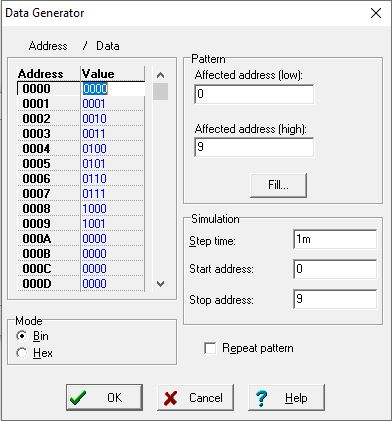
\includegraphics{./res/sig.jpg}
	\caption{Επιλογές γεννήτριας σήματος}
\end{figure}

\subsection{Θεωρητικός υπολογισμός αντιστάσεων}

Για να υπολογίσουμε τις αντιστάσεις $R_1$ έως $R_4$ θα χρησιμοποιήσουμε
τον τύπο για τον υπολογισμού εξόδου του αναστρέφοντα αθροιστή (εφόσον το
πρώτο κύκλωμα είναι ένας αναστρέφων αθροιστής):

\[V_o = - \Big{(}\frac{R_f}{R_1} \cdot V_1 + \frac{R_f}{R_2} \cdot V_2 +
\frac{R_f}{R_3} \cdot V_3 + \frac{R_f}{R_4} \cdot V_4 \Big{)}\]

Εφόσον όμως έχουμε 4 αγνώστους, μπορούμε να λύσουμε ως προς τις εισόδους που
έχουνε 3 μηδενικά και 1 άσσο, δηλαδή τις εισόδους 0001, 0010, 0100 και 1000,
ώστε να εξαλλείψουμε τα περισσότερα μέρη της εξίσωσης και να έχουμε μόνο ένα
άγνωστο. Εν ολίγοις, για κάθε είσοδο, η εξίσωση θα είναι της μορφής (για
ευκολία έχω βγάλει το μείον στην αρχή της εξίσωσης):

\[V_o = \frac{R_f}{R_i} \cdot V_i\]

Η τιμή της $R_f$ θα είναι $\SI{1}{\kohm}$. Μπορεί να είναι οποιαδήποτε άλλη
τιμή.

Θεωρούμε ότι οι τάσεις εισόδου είναι TTL λογικής, δηλαδή $0 = \SI{0}{\volt}$
και $1 = \SI{5}{\volt}$ \\

Για $V_{in} = 0001$:

\[V_o = \frac{R_f}{R_1} \cdot V_1 \Rightarrow
\SI{1}{\volt} = \frac{\SI{1}{\kohm}}{R_1} \cdot \SI{5}{\volt} \Rightarrow
\SI{1}{\volt} = \frac{\SI{5}{\kohm}}{R_1} \Rightarrow
R_1 = \SI{5}{\kohm}\]

Για $V_{in} = 0010$:

\[V_o = \frac{R_f}{R_2} \cdot V_2 \Rightarrow
\SI{2}{\volt} = \frac{\SI{1}{\kohm}}{R_2} \cdot \SI{5}{\volt} \Rightarrow
\SI{2}{\volt} = \frac{\SI{5}{\kohm}}{R_2} \Rightarrow
R_2 = \SI{2.5}{\kohm}\]

Για $V_{in} = 0100$:

\[V_o = \frac{R_f}{R_3} \cdot V_3 \Rightarrow
\SI{4}{\volt} = \frac{\SI{1}{\kohm}}{R_3} \cdot \SI{5}{\volt} \Rightarrow
\SI{4}{\volt} = \frac{\SI{5}{\kohm}}{R_3} \Rightarrow
R_3 = \SI{1.25}{\kohm}\]

Για $V_{in} = 1000$:

\[V_o = \frac{R_f}{R_4} \cdot V_4 \Rightarrow
\SI{8}{\volt} = \frac{\SI{1}{\kohm}}{R_4} \cdot \SI{5}{\volt} \Rightarrow
\SI{8}{\volt} = \frac{\SI{5}{\kohm}}{R_4} \Rightarrow
R_4 = \SI{625}{\ohm}\]

\subsection{Πρακτικός υπολογισμός αντιστάσεων}

Επειδή οι παραπάνω τιμές αντιστάσεων δεν υπάρχουν, θα χρησιμοποιήσουμε τυπικές
τιμές αντιστάσεων της σειράς E96.

\begin{itemize}
	\item Τιμή: $\SI{499}{\ohm}$, $R_1 = \SI{4.99}{\kohm}$
	\item Τιμή: $\SI{249}{\ohm}$, $R_2 = \SI{2.49}{\kohm}$
	\item Τιμή: $\SI{124}{\ohm}$, $R_3 = \SI{1.24}{\kohm}$
	\item Τιμή: $\SI{619}{\ohm}$, $R_4 = \SI{619}{\ohm}$
\end{itemize}

Συνδεσμολογούμε το κύκλωμα αυτή τη φορά με τις τυπικές τιμές αντιστάσεων:

\begin{figure}[H]
	\centering
	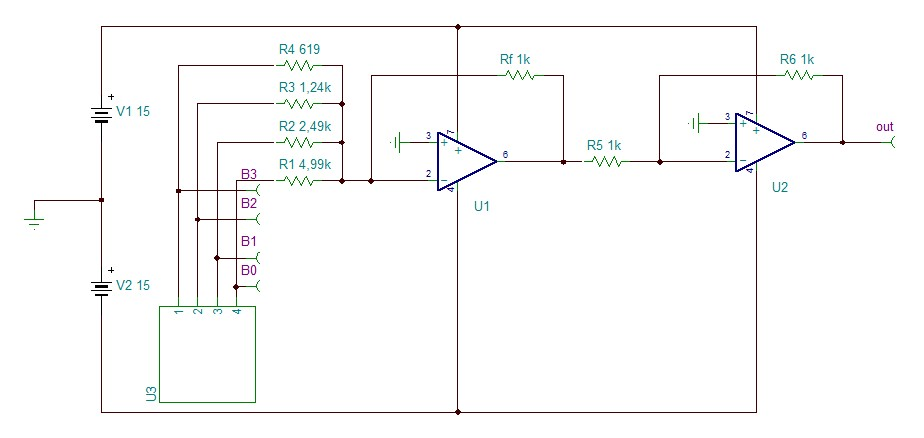
\includegraphics[width=\linewidth]{./res/schem_pract.jpg}
	\caption{4bit μετατροπέας BCD σε αναλογικό με τυπικές αντιστάσεις}
\end{figure}

\subsection{Πίνακας μετρήσεων εξόδου}

Για την μέτρηση της διαφοράς θα αφαιρέσουμε την θεωρητική έξοδο με την πρακτική
έξοδο (σε απόλυτη τιμή):

\[Δ = \lvert V_{th} - V_{pr} \lvert\]

Παρατηρούμε ότι στις περισσότερες εξόδους υπάρχει μικρή διαφορά. Αυτό οφείλεται
στο ότι 1) δεν χρησιμοποιούμε ιδανικά υλικά και 2) οι τυπικές τιμές των
αντιστάσεων είναι όλες, αν και λίγο, διαφορετικές, οπότε το αποτέλεσμα είναι
αναμενόμενο να είναι διαφορετικό:

\begin{center}
\begin{tabular}{|p{3cm}|p{3cm}|l|l|}
	\hline
	\textbf{Δεκαδικός αριθμός} & \textbf{Μετρούμενη τάση} & \textbf{Διαφορά} & \textbf{BCD} \\   	
	\hline
	0 & 0 & $\lvert 0-0 \lvert = 0$ & 0000 \\
	\hline
	1 & 1 & $\lvert 1-1 \lvert = 0$ & 0001 \\
	\hline
	2 & 2 & $\lvert 2-2.01 \lvert = 0.01$ & 0010 \\
	\hline
	3 & 3 & $\lvert 3-3.01 \lvert = 0.01$ & 0011 \\
	\hline
	4 & 4 & $\lvert 4-4.03 \lvert = 0.03$ & 0100 \\
	\hline
	5 & 5 & $\lvert 5-5.03 \lvert = 0.03$ & 0101 \\
	\hline
	6 & 6 & $\lvert 6-6.04 \lvert = 0.04$ & 0110 \\
	\hline
	7 & 7 & $\lvert 7-7.04 \lvert = 0.04$ & 0111 \\
	\hline
	8 & 8 & $\lvert 8-8.06 \lvert = 0.06$ & 1000 \\
	\hline
	9 & 9 & $\lvert 9-9.07 \lvert = 0.07$ & 1001 \\
	\hline
\end{tabular}
\end{center}

\subsection{Γράφημα εξόδου}

Οι διαφορές στην έξοδο μεταξύ θεωρητικών και τυπικών αντιστάσεων είναι πολύ
μικρές, όπως φαίνεται και από τον παραπάνω πίνακα.

\begin{figure}[H]
	\centering
	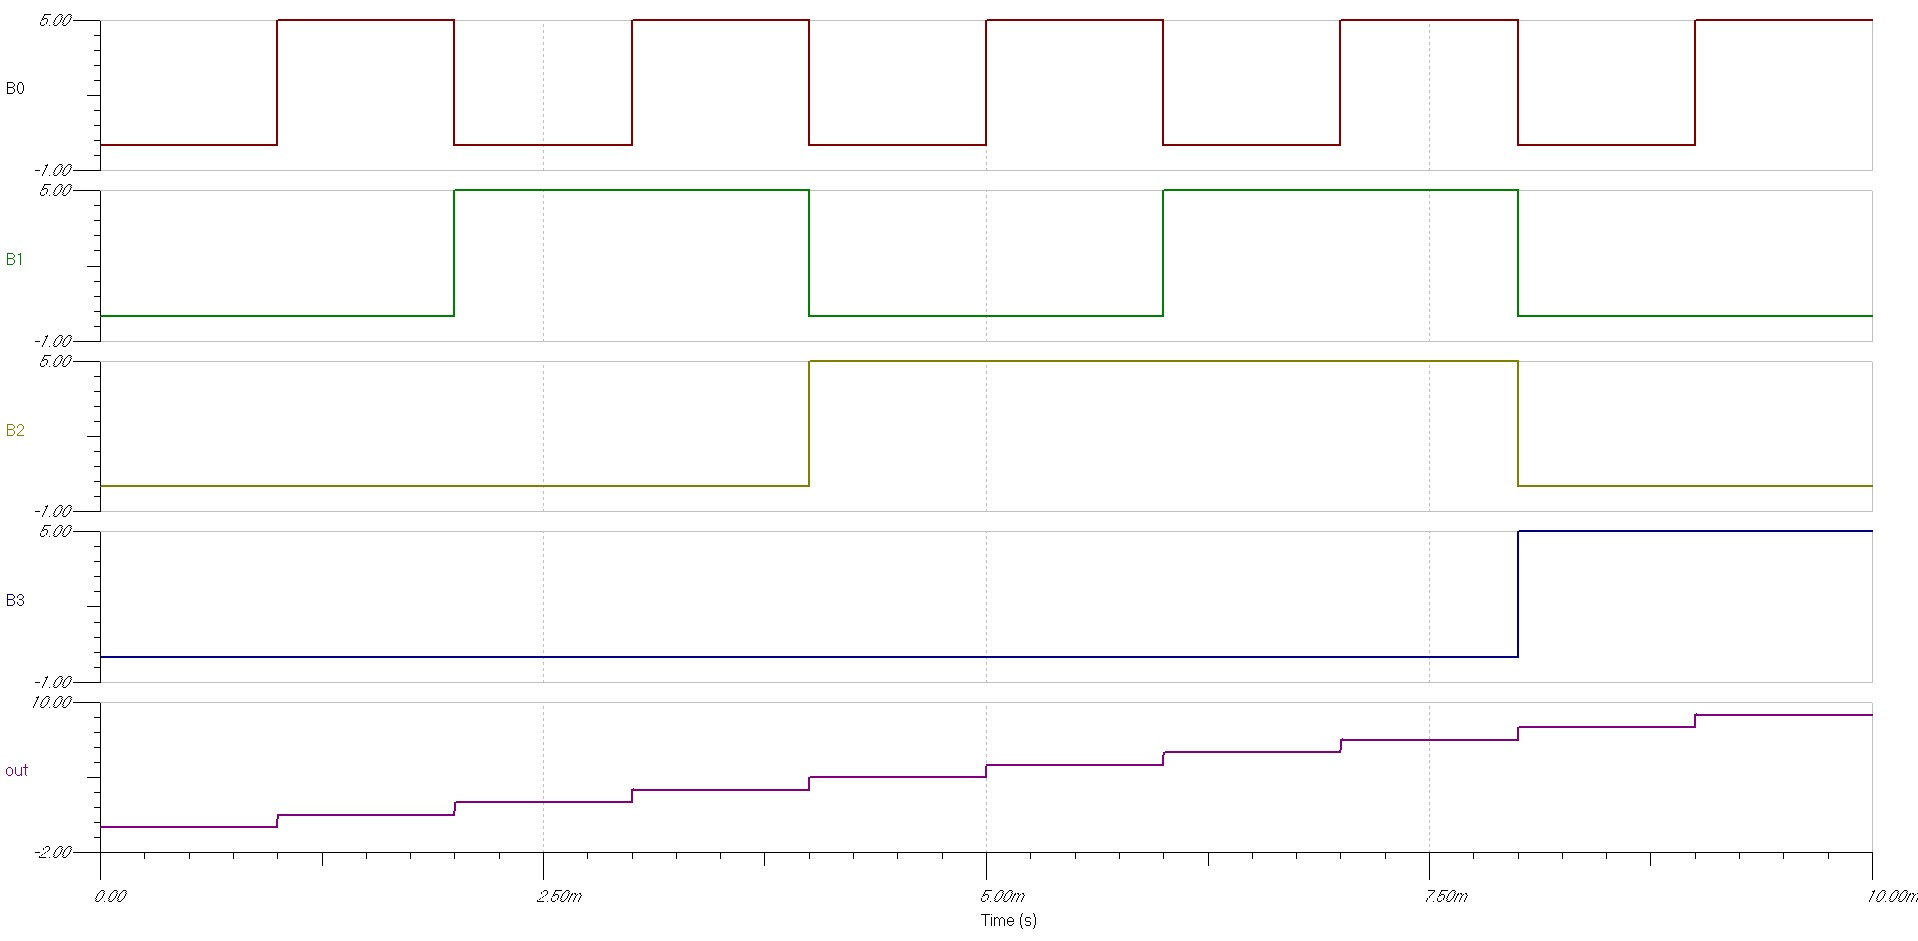
\includegraphics[width=\linewidth]{./res/theoretical.jpg}
	\caption{'Εξοδος με θεωρητικές αντιστάσεις}
\end{figure}

\begin{figure}[H]
	\centering
	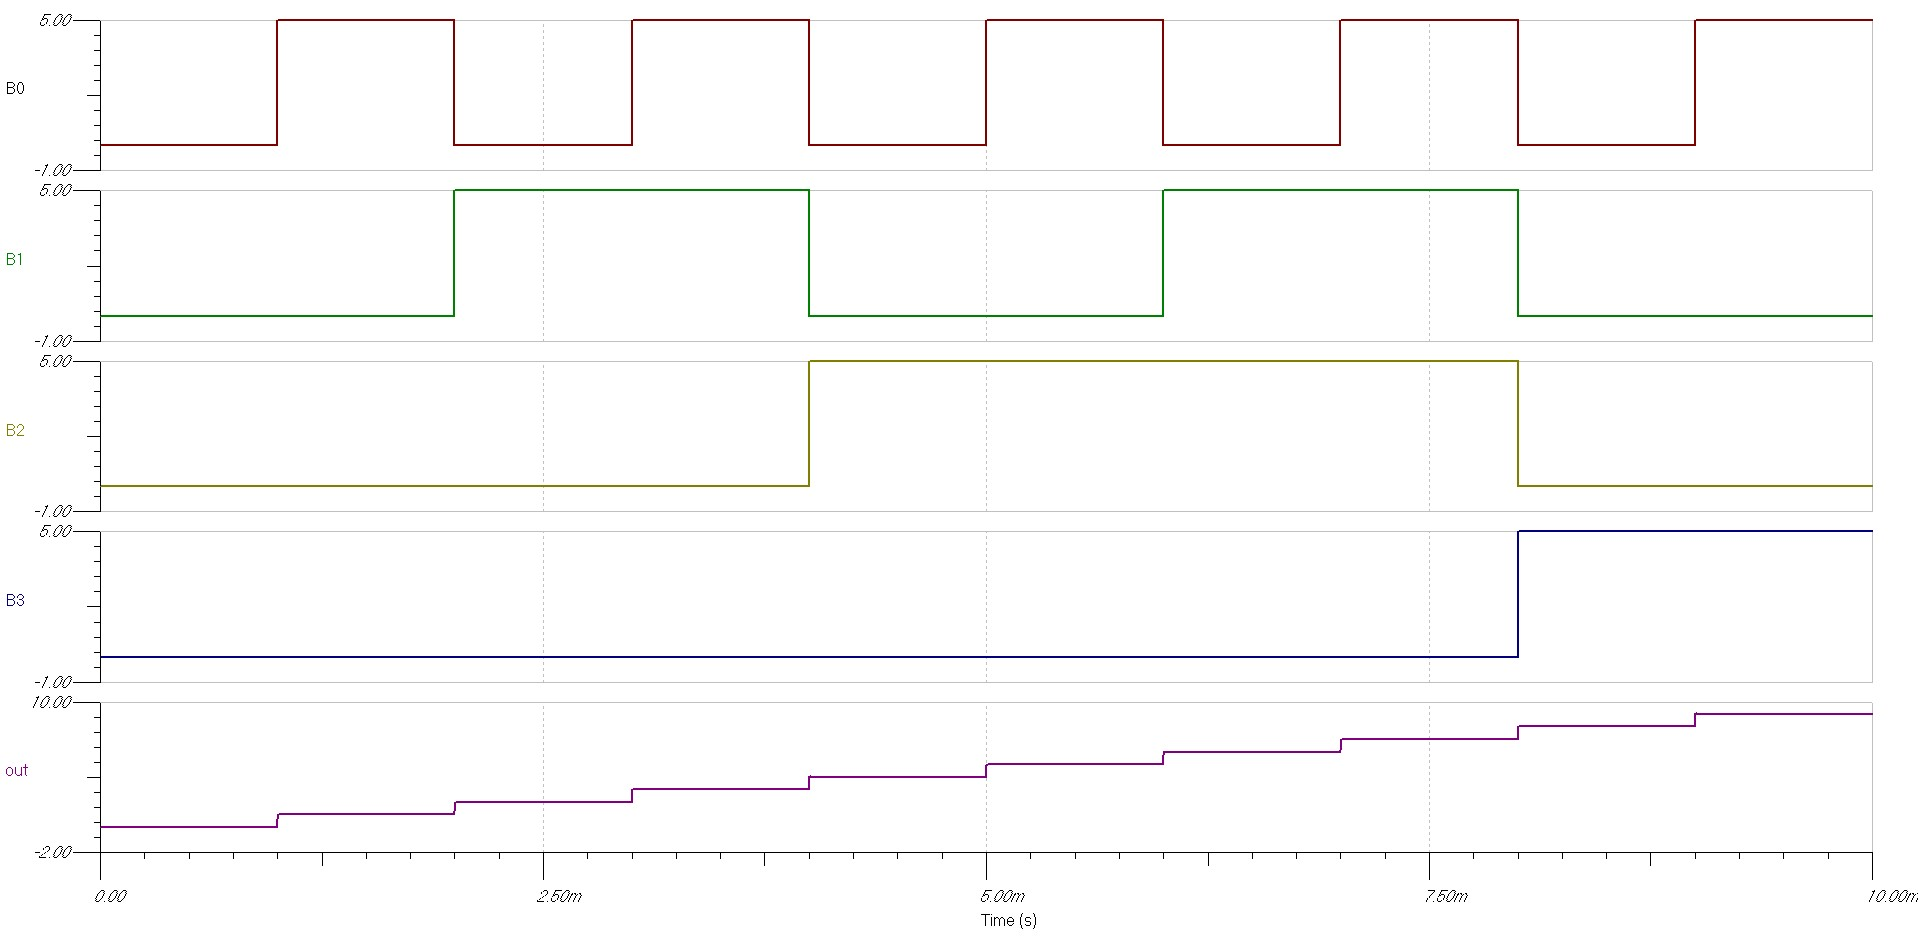
\includegraphics[width=\linewidth]{./res/practical.jpg}
	\caption{'Εξοδος με τυπικές αντιστάσεις}
\end{figure}

\section{Υλοποίηση σε breadboard}

\begin{itemize}
	\item Παρουσιάστε το κύκλωμά σας υλοποιημένο σε breadboard μέσω
		της εφαρμογής Tinkercad.
\end{itemize}

%\begin{figure}[H]
	%\centering
	%\includegraphics[width=\linewidth]{./res/<++>.jpg}
%\end{figure}

\end{document}
